\documentclass[serif,mathserif]{beamer}
\usepackage{graphicx}
\usepackage[utf8]{inputenc}
\usepackage[frenchb]{babel}
\usepackage{color}
\usepackage{beamerthemesplit}

\definecolor{Silver1}{RGB}{0,93,117}
\definecolor{Silver2}{RGB}{50,50,50}
\definecolor{Silver3}{RGB}{0,142,178}


\setbeamercolor{frametitle}{use=structure,fg=white,bg=Silver1}
\setbeamercolor{structure}{fg=Silver3}
\setbeamercolor{section in head/foot}{bg=Silver2}
\setbeamercolor{author in head/foot}{bg=Silver2}
\setbeamercolor{date in head/foot}{fg=Silver2}



%%%%%%%%%%%%%%%%%%%%%%%UNIVERSITY LOGO DEFINITION%%%%%%%%%%%%%%%%%%%%%

\usepackage[absolute,overlay]{textpos}
  \setlength{\TPHorizModule}{1mm}
  \setlength{\TPVertModule}{1mm}
\newcommand{\logoUniv}{
	\begin{textblock}{0}(115,22,5)
      
\includegraphics[scale=0.12,viewport=0 0 0 0]{angers.png}
    \end{textblock}	
}


%%%%%%%%%%%%%%%%%%%%%%%%%%%%PRESENTATION PAGE%%%%%%%%%%%%%%%%%%%%%%%%%


\title[CUDAisation\hspace{12,5em}\insertframenumber/\inserttotalframenumber]{CUDAisation du code impératif}
\date{Vendredi 03 juin 2016} %leave out for today's date to be insterted

\institute[UFR Sciences]{Université d'Angers}


\begin{document}

\begin{frame}[plain]
\maketitle
\scriptsize

	\begin{minipage}{0.49\textwidth} 
		\begin{flushleft}
			\textbf{Tuteur pédagogique}:Jean Michel RICHER
    	\end{flushleft}
    \end{minipage}
    \begin{minipage}{0.49\textwidth} 
		\begin{flushright}
		Alexis BRIARD\\
		Jason JAMET\\
		Guillaume GRANDJEAN	
    		\end{flushright}
    \end{minipage}

\end{frame}
%%%%%%%%%%%%%%%%%%%%%%%%%%%%TABLE OF CONTENT%%%%%%%%%%%%%%%%%%%%%%%%%%


\frame{
	\frametitle{Plan} 
	\logoUniv \footnotesize
	\tableofcontents 
}
%%%%%%%%%%%%%%%%%%%%%%%%%%%%%%%% codaCudaTransforme.png SLIDES%%%%%%%%%%%%%%%%%%%%%%%%%%%%%%%%

\section{Présentation} 
\subsection{Objectif}
\frame{\frametitle{Objectif} \logoUniv
\begin{itemize}
\item Transformer un code impératif en CUDA
\end{itemize}
~~\\~~\\~~\\~~\\~~\\

	\begin{textblock}{0}(2,70)
      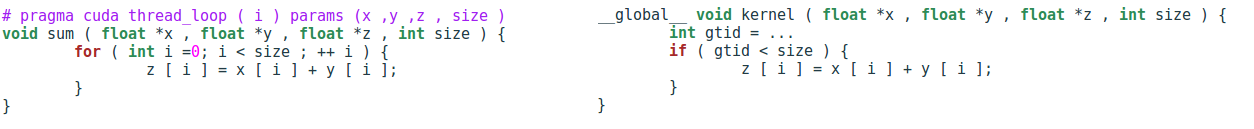
\includegraphics[scale=0.38,viewport=0 0 0 0]{codaCudaObjectif.png}
    \end{textblock}	
}


\section{Analyse du problème}
\subsection{Analyse générale}
\frame{\frametitle{Analyse générale} \logoUniv

\begin{block}{Les transformations à réaliser :}
\begin{itemize}
\item Initialisation de la variable récupérée dans le thread\_loop
\item Remplacement de la boucle for en condition if
\item Modification de l'entête de la fonction
\end{itemize} 
\end{block}

}

\frame{\frametitle{Analyse générale} \logoUniv

\begin{block}{Eléments qui peuvent poser problème :}
\begin{itemize}
\item La variable size
\item La taille des blocs
\item Recherche de la boucle à paralléliser
\end{itemize} 
\end{block}

\begin{block}{Informations à extraire du code :}
\begin{itemize}
\item Pragma
\item Boucle for
\item Déclaration de variables
\item Fonction non void
\end{itemize} 
\end{block}
}






\subsection{Solutions envisagées}
\frame{\frametitle{Solutions envisagées}  \logoUniv
 
\begin{block}{Les solutions:}
\begin{itemize}
\item Analyseur syntaxique / lexical
\item Compilateur gcc
\item Regex
\end{itemize}
\end{block}

}

\section{Conception}
\subsection{Solution retenue}
\frame{\frametitle{Solution retenue}  \logoUniv
\begin{block}{Analyseur syntaxique / lexical}
 Simple d'utilisation, maitrisé par les membres de l'équipe.
\end{block}
~~\\~~\\
\begin{center}
      
\includegraphics[scale=0.38]{flexBison.png}
\end{center}	


}
\subsection{Réalisation}
\frame{\frametitle{Base de travail et correction}  \logoUniv
	\begin{itemize}
		\item 1ère version from scratch
		\item 2nd version basée sur l'implémentation yacc/lex de Jeff Lee
		\item 3ème version basée sur le projet "tc-parser" (github)
	\end{itemize}
}
\frame{\frametitle{Analyse du pragma}  \logoUniv
	\begin{itemize}
		\item Définition du format
		\item Modification de l'arbre
	\end{itemize}
	
	{\color{red}\#pragma cuda} {\color{blue}thread\_loop(j)} {\color{orange}block\_size(2,2)} {\color{purple}nbr\_threads(16)}
}

\frame{\frametitle{Recherche de la boucle à paralléliser} \logoUniv
	\begin{itemize}
		\item Parcours de la fonction à CUDAiser
		\item Recherche du thread\_loop dans les paramètre des boucles for
	\end{itemize}
	\begin{center}
      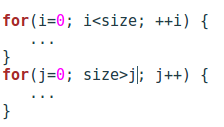
\includegraphics[scale=0.45]{for.png}
	\end{center}	
}

\frame{\frametitle{Vérification de la portée des variables}\logoUniv
	\begin{itemize}
		\item Accessibilité des variables
	\end{itemize}
	

}

\frame{\frametitle{Transformation de la fonction}  \logoUniv
\begin{itemize}
\item Modification de l'entête de la fonction
\item Modification de l'initialisation de la variable sur la quelle itérer
\item Modification de la boucle for vers une condition if
\end{itemize} 


}

\frame{\frametitle{Wrapper de la fonction transformée}  \logoUniv
\begin{itemize}
\item Fonction qui appelle le kernel généré
\item Récupération des paramètres contenus dans le pragma
\item Affectation selon les paramètres s'ils existent
\end{itemize} 

}

\section{Améliorations}
\subsection{Améliorations}
\frame{\frametitle{Améliorations}  \logoUniv
\begin{itemize}
\item Parse complet du langage c
\item Gestion plus complète de la boucle for
\item Automatisation des allocations
\end{itemize} 
}
\end{document}

